\documentclass[9pt,a4paper]{extarticle}
\usepackage[margin=1.55cm]{geometry}
\usepackage{fontspec}
\setmainfont{Times New Roman}
\setmonofont{Consolas}[Scale=0.86]
\usepackage{amsmath,amssymb}
\usepackage{booktabs,longtable,array,calc}
\usepackage{graphicx}
\setkeys{Gin}{keepaspectratio}
\usepackage[hidelinks]{hyperref}
\usepackage{float}
\providecommand{\tightlist}{\setlength{\itemsep}{0pt}\setlength{\parskip}{0pt}}
\setlength{\parskip}{3.2pt}
\setlength{\parindent}{0pt}
\setlength{\tabcolsep}{3.2pt}
\renewcommand{\arraystretch}{1.05}
\linespread{1.015}
\emergencystretch=1em
\setcounter{secnumdepth}{0}
\setcounter{tocdepth}{0}
\title{Capacity-Constrained CVRP Clustering on an Analog Neutral-Atom Register}
\author{Track A Report — DuQuantum Hackathon — Team Qualies}
\date{2026-10-25}
\begin{document}
\maketitle
\vspace{-1.8em}
\section{Abstract}\label{abstract}

This work investigates a cluster-first decomposition of the capacitated
vehicle-routing problem (CVRP) for an analog neutral-atom processor.
Customer-to-vehicle assignment is encoded with one atom per binary
decision, after which each selected cluster is routed exactly. The
resulting formulation requires 8, 30, and 60 atoms on tiers S, M, and L,
respectively. Raw quantum sampling is reliable on tier S, substantially
less accurate on tier M, and rarely feasible on tier L. A held-out
capacity study shows that a stronger load-balance coefficient can
improve average feasibility, albeit with instance-dependent degradation
in route quality. A depot-aware classical clustering surrogate
substantially reduces the decomposition loss on tier L, whereas
deterministic repair provides no advantage over identically processed
random one-hot controls. These findings distinguish errors arising from
the clustering objective, capacity penalization, geometric embedding,
and quantum sampling.

\section{1. Mathematical formulation}\label{mathematical-formulation}

\textbf{Formulation overview.} The register determines which customers
share a vehicle, and each resulting cluster is routed exactly. One atom
is assigned to each customer--vehicle pair.

\textbf{Rationale for cluster-first decomposition.} Encoding the full
route (customer, vehicle, position) requires approximately \(N^2K\)
atoms: 32 / 300 / 900 for S / M / L, against 80 available (DERIVATIONS
Q1). Deciding only the grouping needs \(NK\). The cost is a
\emph{decomposition gap}: the best grouping under our objective is not
always the grouping of the shortest routes. It is 0 \% on 5 of 11
instances and up to 21.7 \% on the rest (§5, decomposition table).

\textbf{Decision variables.} Let \(N\) denote the number of customers
with demands \(d_i\), \(K\) the number of identical vehicles of capacity
\(Q\), and \(d_{ij}\) the distance between customers \(i\) and \(j\).
The bit \(x_{ik}=1\) means customer \(i\) rides on vehicle \(k\). A
valid grouping has exactly one \(1\) in every customer's row
(``one-hot'').

\textbf{Clustering objective.} Spatially compact groups are encouraged
by summing the distances between every pair of customers that share a
vehicle: \begin{equation}
f(x)=\sum_{k=1}^{K}\ \sum_{i<j} d_{ij}\,x_{ik}\,x_{jk}.
\end{equation} This surrogate introduces the decomposition gap reported
below. Its additivity permits exact certification of the model optimum
by dynamic programming (\texttt{cvrp/exact.py}).

\textbf{Assignment constraint.} The requirement that every customer be
assigned to exactly one vehicle is enforced by a squared penalty with
weight \(A\): \begin{equation}
A\sum_{i=1}^{N}\Big(1-\sum_{k=1}^{K}x_{ik}\Big)^2 .
\end{equation} Expansion produces a uniform linear term \(-A\) and
coupling \(+2A\) between the \(K\) atoms of each customer. No additional
atoms are required, although \(A\) becomes the largest coupling that the
register must realize.

\textbf{Capacity constraint.} For vehicle load
\(L_k=\sum_i d_i x_{ik}\le Q\), the formulation uses unbalanced
penalization (Montañez-Barrera et al.~2024),
\(\sum_k\big[-\lambda_1(Q-L_k)+\lambda_2(Q-L_k)^2\big]\), because it
needs no slack atoms. On one-hot strings its linear part is the same
constant for every valid grouping, so it drops out together with
\(\lambda_1\) (the ``one-hot identity'', DERIVATIONS §4); what survives
is a load-balance term \begin{equation}
\lambda_2\sum_{k=1}^{K} L_k^2 \;=\; \text{const}+2\lambda_2\sum_k\sum_{i<j} d_i d_j\,x_{ik}x_{jk}.
\end{equation} The balance term \emph{alone} has a feasible minimiser
for \(K=2\) whenever a feasible split exists; adding the distance
objective removes that guarantee, and no such guarantee exists for
\(K\ge3\). We therefore score feasible decodes only.

\textbf{Distinction among optimization objectives.} The constrained
problem minimizes Eq. (1) subject to both constraints. The QUBO sent to
the embedder is, up to the offset \(AN\), \begin{equation}
E(x)=-A\sum_{ik}x_{ik}+2A\sum_i\sum_{k<\ell}x_{ik}x_{i\ell}
+\sum_k\sum_{i<j}(d_{ij}+2\lambda_2d_id_j)x_{ik}x_{jk}.
\end{equation} The device realises
\(E_{\mathrm{dev}}(x)=-\delta_f\sum_a x_a+\sum_{a<b}U_{ab}x_ax_b\).
Positive couplings and uniform linear terms make the QUBO compatible in
sign, but planar \(U_{ab}=C_6/r_{ab}^6\) still approximates it.

\textbf{Penalty coefficients.}
\(A=\max_i\sum_{j\ne i}(d_{ij}+2\lambda_2 d_id_j)+1\), which guarantees
that every minimizer is one-hot (DERIVATIONS §4).
\(\lambda_2=0.15\,R/(2Q)\) with \(R=\max_i\sum_j d_{ij}\), from a
40-seed brute-force scan. Brute force on the five S instances: the
minimiser is feasible and optimal on 5/5; \(A\) survives one halving and
fails at \(A/4\); \(\lambda_2\) is not binding on any S instance.

\section{2. Resource requirements and
instances}\label{resource-requirements-and-instances}

\begin{longtable}[]{@{}
  >{\raggedright\arraybackslash}p{(\linewidth - 10\tabcolsep) * \real{0.1667}}
  >{\raggedright\arraybackslash}p{(\linewidth - 10\tabcolsep) * \real{0.1667}}
  >{\raggedright\arraybackslash}p{(\linewidth - 10\tabcolsep) * \real{0.1667}}
  >{\raggedright\arraybackslash}p{(\linewidth - 10\tabcolsep) * \real{0.1667}}
  >{\raggedright\arraybackslash}p{(\linewidth - 10\tabcolsep) * \real{0.1667}}
  >{\raggedright\arraybackslash}p{(\linewidth - 10\tabcolsep) * \real{0.1667}}@{}}
\toprule\noalign{}
\begin{minipage}[b]{\linewidth}\raggedright
Encoding
\end{minipage} & \begin{minipage}[b]{\linewidth}\raggedright
count
\end{minipage} & \begin{minipage}[b]{\linewidth}\raggedright
S
\end{minipage} & \begin{minipage}[b]{\linewidth}\raggedright
M
\end{minipage} & \begin{minipage}[b]{\linewidth}\raggedright
L
\end{minipage} & \begin{minipage}[b]{\linewidth}\raggedright
fits 80?
\end{minipage} \\
\midrule\noalign{}
\endhead
\bottomrule\noalign{}
\endlastfoot
assignment variables only & \(NK\) & 8 & 30 & 60 & yes \\
+ binary slack (textbook) & \(NK+K\lceil\log_2(Q{+}1)\rceil\) & 14 & 45
& 80 & yes (L = cap) \\
\textbf{ours} (\texttt{onehot-ub}) & \(NK\) & \textbf{8} & \textbf{30} &
\textbf{60} & yes \\
\end{longtable}

Tiers: S \(N{=}4,K{=}2,Q{=}7\); M \(N{=}10,K{=}3,Q{=}20\); L
\(N{=}15,K{=}4,Q{=}30\) (\texttt{scripts/variable\_count.py}). We save 6
/ 15 / 20 atoms over the textbook encoding and never discard a readout
bit.

\textbf{Instances.} A seeded generator first draws a balanced assignment
and then draws demands within each vehicle's remaining capacity; that
assignment is the shipped certificate and the validator rechecks it.
Locations are uniform in \([0,100]^2\) and the depot is fixed at
\((50,50)\). Across S/M/L, \(\rho\) ranges are 0.643--0.857 /
0.700--0.950 / 0.600--0.708 and \(d_{\max}/Q\) ranges are 0.429--0.571 /
0.400 / 0.300--0.333.

\section{3. Geometric embedding (DERIVATIONS
§5)}\label{geometric-embedding-derivations-5}

\textbf{Embedding strategy.} A generic least-squares placement does not
realize the rook's graph with sufficient accuracy. The adopted method
therefore fits device energies on one-hot strings. On the five tested S
instances the realised register preserves the optimal clustering; it
does not reproduce every model energy exactly. On M/L it fails to
preserve the ordering of groupings.

\textbf{Limitations of generic placement.} The \(K\) atoms representing
one customer must be separated by 5 µm to form the required clique. Any
atom of another customer is then at nearly the same distance from all
\(K\) of them, so the couplings that should be zero (different customer
\emph{and} different vehicle) come out as large as the wanted ones.
Measured: relative coupling error 0.95, defined as
\(\|U/\alpha-J\|_F/\|J\|_F\) over all pairs (lower is better;
\texttt{cvrp/embed.py}), and on S\_seed04 the register's ground state
was an infeasible string.

\textbf{One-hot-subspace fitting.} On a one-hot string, each pair of
customers has exactly one active coupling; consequently, only the
difference \emph{same-vehicle minus cross-vehicle} has to match the
model (DERIVATIONS 5.7b); the cross couplings only need to be constant.
Each customer becomes a rigid 5 µm \(K\)-gon, which realises the clique
exactly with \(\alpha=C_6/(5\,\mu\text{m})^6/2A\); the centres and
orientations are fitted (L-BFGS, 6 seeded starts) so that the device
energies of all one-hot strings match \(\alpha\,E_\text{QUBO}\), with
single-flip defects forced above their parents and the final detuning
\(\delta_f\) as a fit parameter. Registers are committed in
\texttt{embeddings/}; every run checks the realised register (is its own
minimiser feasible and optimal? smallest defect gap). Tier S: 5/5 yes,
coupling error 0.21--0.32.

\begin{figure}[H]
\centering
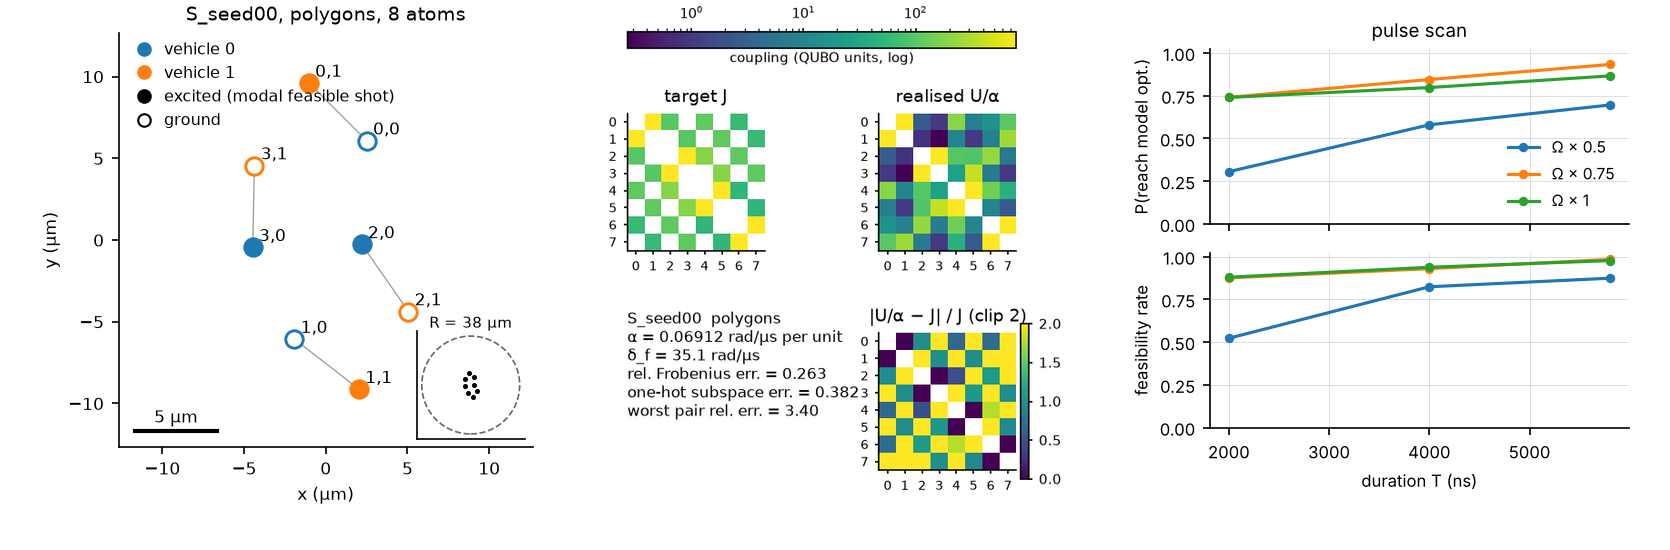
\includegraphics[width=0.96\linewidth,height=\textheight,keepaspectratio]{report/figures/overview.png}
\caption{Left: S\_seed00 register and modal feasible sample. Middle:
target and realized couplings; the one-hot-subspace error is 0.382.
Right: tier-S pulse scan; 0.75 times maximum amplitude at 5800 ns
performs best among the tested settings.}
\end{figure}

\textbf{An isolated-polygon bound.} Ignoring other polygons, one atom of
a \(K\)-gon excited costs \(-\delta_f\); two excited cost
\(-2\delta_f+U_{\min}\), where \(U_{\min}\) is the coupling of the
\emph{weakest} pair inside the polygon. One one excitation is preferred
only if \begin{equation}
0<\delta_f<U_{\min}.
\end{equation} For \(K\le3\) every pair is the 5 µm side,
\(U_{\min}=55.1\) rad/µs; the S fits land at \(\delta_f=35\)--38 rad/µs
(0.64--0.68 \(U_{\min}\)). On M the fit is ill-conditioned and ran to
the device maximum, 125.66 rad/µs \(=2.28\,U_{\min}\), which favours
\emph{two} vehicles per customer; the embedder now enforces Eq. (4)
(fallback \(0.65\,U_{\min}\)). For \(K=4\) a 5 µm square has 7.07 µm
diagonals, and \(1/r^6\) turns that \(\sqrt2\) into a factor 8:
\(U_{\min}=6.9\) rad/µs, so the L registers run at \(\delta_f=4.5\)
rad/µs. Four points in a plane are never equidistant, so a planar
one-hot clique for \(K\ge4\) is never uniform. Interactions with
occupied atoms in other polygons also enter the excitation cost, so Eq.
(5) is useful but not a sufficient global guarantee.

\section{4. Pulse protocol (DERIVATIONS
§6)}\label{pulse-protocol-derivations-6}

\textbf{Selected schedule.} The pulse duration is 5800 ns (200 ns below
the device maximum), with \(\Omega=0.75\,\Omega_{\max}\) and fitted
\(\delta_f\). A three-point \(\Omega\) ramp (15 \% up, 70 \% plateau, 15
\% down) and a linear detuning sweep during the plateau from
\(\delta_0=-\min(\max(|\delta_f|,2\Omega_{\max}),\delta_{\max})\) to
\(\delta_f\). Starting far below resonance puts every atom in
\(|g\rangle\); the positive final detuning and defect-gap fit target one
excitation per customer. Every sequence is built with Pulser on
\texttt{AnalogDevice} and validated against the device object.

\textbf{Parameter selection.} A scan on three S instances (Fig. 1 right;
DERIVATIONS §6.6) was evaluated by P(reach), best gap, and feasibility
rather than mean cost. Performance improves with duration at every
\(\Omega\) (2000 → 4000 → 5800 ns); \(0.75\,\Omega_{\max}\) exceeds full
and half power at 4000 and 5800 ns; \(\delta_f\times\{0.8,1,1.25\}\)
gives 0.915 / 0.932 / 0.884, so the fitted value is retained.
S\_seed02/03, not used in the scan, reach the model optimum in 99 \% /
96 \% of samples with these settings. Emulators: pulser-simulation
(QuTiP) for every S headline row; emu-sv cross-check on S\_seed00 (0.96
vs 0.94); an in-house exact state-vector integrator built from Pulser's
own samples for the scans (total-variation distance 0.05--0.07 from
QuTiP at 500 shots, i.e.~sampling noise); emu-mps for M and L with the
bond dimension recorded.

\section{\texorpdfstring{5. Results (brief Table 3; complete table:
\texttt{results.csv}, 79
rows)}{5. Results (brief Table 3; complete table: results.csv, 79 rows)}}\label{results-brief-table-3-complete-table-results.csv-79-rows}

\textbf{Evaluation metrics.} The table reports raw samples without
repair. \emph{feas.} denotes the fraction of samples that decode to a
capacity-feasible grouping. \emph{model gap}: best feasible shot against
the exact model optimum; \emph{CVRP gap}: that shot routed exactly
against \(C^*\) (proven on S, best known on M/L); both on feasible
decodes only, ``undefined'' if there are none. \emph{P(reach \(C^*\))}:
shots whose grouping routes to \(C^*\), so it includes the decomposition
loss. \emph{P(gap ≤ 5 \%)}: shots within 5 \% of the model optimum; on
every S instance and on M\_seed00/01 this equals P(reach model optimum)
because the next-best feasible grouping is 11--62 \% worse, on M\_seed02
it does not (six groupings within 5 \%; DERIVATIONS Q-M3).
\emph{fidelity}: relative coupling error of the full matrix, lower is
better.

\begin{longtable}[]{@{}
  >{\raggedright\arraybackslash}p{(\linewidth - 16\tabcolsep) * \real{0.0811}}
  >{\raggedright\arraybackslash}p{(\linewidth - 16\tabcolsep) * \real{0.3243}}
  >{\raggedright\arraybackslash}p{(\linewidth - 16\tabcolsep) * \real{0.0541}}
  >{\raggedright\arraybackslash}p{(\linewidth - 16\tabcolsep) * \real{0.0811}}
  >{\raggedright\arraybackslash}p{(\linewidth - 16\tabcolsep) * \real{0.0811}}
  >{\raggedright\arraybackslash}p{(\linewidth - 16\tabcolsep) * \real{0.0811}}
  >{\raggedright\arraybackslash}p{(\linewidth - 16\tabcolsep) * \real{0.0811}}
  >{\raggedright\arraybackslash}p{(\linewidth - 16\tabcolsep) * \real{0.0676}}
  >{\raggedright\arraybackslash}p{(\linewidth - 16\tabcolsep) * \real{0.1486}}@{}}
\toprule\noalign{}
\begin{minipage}[b]{\linewidth}\raggedright
instance
\end{minipage} & \begin{minipage}[b]{\linewidth}\raggedright
method
\end{minipage} & \begin{minipage}[b]{\linewidth}\raggedright
feas.
\end{minipage} & \begin{minipage}[b]{\linewidth}\raggedright
model gap
\end{minipage} & \begin{minipage}[b]{\linewidth}\raggedright
CVRP gap
\end{minipage} & \begin{minipage}[b]{\linewidth}\raggedright
P(reach C*)
\end{minipage} & \begin{minipage}[b]{\linewidth}\raggedright
P(gap≤5\%)
\end{minipage} & \begin{minipage}[b]{\linewidth}\raggedright
fidelity
\end{minipage} & \begin{minipage}[b]{\linewidth}\raggedright
backend
\end{minipage} \\
\midrule\noalign{}
\endhead
\bottomrule\noalign{}
\endlastfoot
S\_seed00 & ours & 1.00 & 0.0 \% & 0.0 \% & 0.94 & 0.94 & 0.26 &
qutip \\
S\_seed00 & ours, tight A (ablation) & 1.00 & 0.0 \% & 0.0 \% & 0.03 &
0.03 & 0.31 & qutip \\
S\_seed00 & random assignments (one-hot) & 0.63 & 0.0 \% & 0.0 \% & 0.12
& 0.12 & 0.26 & random-onehot \\
S\_seed00 & qubo-solver quantum & 1.00 & 0.0 \% & 0.0 \% & 0.78 & 0.78 &
0.12 & qs-quantum \\
S\_seed00 & qubo-solver tabu & 1.00 & 0.0 \% & 0.0 \% & 1.00 & 1.00 &
undef. & qs-classical \\
S\_seed00 & random sampler & 0.04 & 0.0 \% & 0.0 \% & 0.01 & 0.01 & 0.95
& random \\
S\_seed01 & ours & 0.95 & 0.0 \% & 0.0 \% & 0.95 & 0.95 & 0.21 &
qutip \\
S\_seed02 & ours & 1.00 & 0.0 \% & 0.0 \% & 0.99 & 0.99 & 0.31 &
qutip \\
S\_seed03 & ours & 1.00 & 0.0 \% & 15.6 \% & 0.01 & 0.96 & 0.29 &
qutip \\
S\_seed04 & ours & 1.00 & 0.0 \% & 21.7 \% & 0.02 & 0.89 & 0.32 &
qutip \\
M\_seed00 & ours (emu-mps) & 0.04 & 67.9 \% & 29.9 \% & 0.00 & 0.00 &
0.58 & emu-mps χ=32 \\
M\_seed00 & qubo-solver quantum & 0.02 & 72.1 \% & 35.2 \% & 0.00 & 0.00
& 0.09 & qs-quantum χ=32 \\
M\_seed01 & ours (emu-mps) & 0.39 & 37.9 \% & 9.2 \% & 0.00 & 0.00 &
0.08 & emu-mps χ=32 \\
M\_seed01 & qubo-solver quantum & 0.37 & 47.5 \% & 11.2 \% & 0.00 & 0.00
& 0.08 & qs-quantum χ=32 \\
M\_seed02 & ours (emu-mps) & 0.45 & 23.0 \% & 16.0 \% & 0.00 & 0.00 &
0.47 & emu-mps χ=32 \\
M\_seed02 & qubo-solver quantum & 0.39 & 34.2 \% & 13.6 \% & 0.00 & 0.00
& 0.09 & qs-quantum χ=32 \\
L\_seed00 & ours (emu-mps) & 0.01 & 140.0 \% & 79.7 \% & 0.00 & 0.00 &
0.65 & emu-mps χ=32 \\
L\_seed01 & ours (emu-mps) & 0.00 & 182.9 \% & 75.1 \% & 0.00 & 0.00 &
0.65 & emu-mps χ=32 \\
L\_seed02 & ours (emu-mps) & 0.00 & undef. & undef. & 0.00 & 0.00 & 0.64
& emu-mps χ=32 \\
\end{longtable}

(Source: \texttt{scripts/report\_tables.py}, generated from
\texttt{results.csv}. Values are raw samples; repair and additional
control rows remain in \texttt{results.csv}; the full control block is
shown only for S\_seed00)

\textbf{Reference \(C^*\) (brief §9.3).} CPLEX is not importable, so
\(C^*\) is the best of qubo-solver's simulated annealing on our
penalized QUBO and our constrained annealing on the CVRP, each 10 seeded
restarts with a 60 s max solve time (settings in
\texttt{instances/*.json}). On S the exhaustive dynamic programme is
also run and agrees 5/5, so S references are proven; M/L are best known.
The QUBO-side annealer reaches \(C^*\) on 5/5 S and 2/3 M instances but
stays 23--34 \% above it on all three L (599.9 / 554.6 / 521.7 vs 447.0
/ 434.9 / 424.7). The reported \(C^*\) values therefore do not rely
exclusively on the QUBO annealer.

\begin{longtable}[]{@{}
  >{\raggedright\arraybackslash}p{(\linewidth - 8\tabcolsep) * \real{0.2000}}
  >{\raggedright\arraybackslash}p{(\linewidth - 8\tabcolsep) * \real{0.2000}}
  >{\raggedright\arraybackslash}p{(\linewidth - 8\tabcolsep) * \real{0.2000}}
  >{\raggedright\arraybackslash}p{(\linewidth - 8\tabcolsep) * \real{0.2000}}
  >{\raggedright\arraybackslash}p{(\linewidth - 8\tabcolsep) * \real{0.2000}}@{}}
\toprule\noalign{}
\begin{minipage}[b]{\linewidth}\raggedright
instance
\end{minipage} & \begin{minipage}[b]{\linewidth}\raggedright
ρ
\end{minipage} & \begin{minipage}[b]{\linewidth}\raggedright
C* (best known)
\end{minipage} & \begin{minipage}[b]{\linewidth}\raggedright
model optimum routed exactly
\end{minipage} & \begin{minipage}[b]{\linewidth}\raggedright
decomposition gap
\end{minipage} \\
\midrule\noalign{}
\endhead
\bottomrule\noalign{}
\endlastfoot
S\_seed00 & 0.714 & 262.97 & 262.97 & 0.0 \% \\
S\_seed01 & 0.857 & 245.02 & 245.02 & 0.0 \% \\
S\_seed02 & 0.714 & 254.62 & 254.63 & 0.0 \% \\
S\_seed03 & 0.643 & 197.44 & 228.34 & 15.6 \% \\
S\_seed04 & 0.714 & 184.42 & 224.49 & 21.7 \% \\
M\_seed00 & 0.950 & 432.00 & 432.00 & 0.0 \% \\
M\_seed01 & 0.733 & 368.36 & 368.36 & 0.0 \% \\
M\_seed02 & 0.700 & 360.86 & 385.62 & 6.9 \% \\
L\_seed00 & 0.650 & 446.97 & 525.71 & 17.6 \% \\
L\_seed01 & 0.708 & 434.91 & 470.67 & 8.2 \% \\
L\_seed02 & 0.600 & 424.66 & 480.17 & 13.1 \% \\
\end{longtable}

\textbf{Model selection, evaluated classically.} Each additive objective
below is solved exactly with capacity enforced and its groups are then
routed exactly. These numbers test objective quality only; the
alternatives have not been mapped to the analog register.
\texttt{depot-MST} means \(\operatorname{MST}(S)+2\min_{i\in S}d_{0i}\)
per group.

\begin{longtable}[]{@{}
  >{\raggedright\arraybackslash}p{(\linewidth - 6\tabcolsep) * \real{0.2500}}
  >{\raggedright\arraybackslash}p{(\linewidth - 6\tabcolsep) * \real{0.2500}}
  >{\raggedright\arraybackslash}p{(\linewidth - 6\tabcolsep) * \real{0.2500}}
  >{\raggedright\arraybackslash}p{(\linewidth - 6\tabcolsep) * \real{0.2500}}@{}}
\toprule\noalign{}
\begin{minipage}[b]{\linewidth}\raggedright
tier
\end{minipage} & \begin{minipage}[b]{\linewidth}\raggedright
pairwise routed gaps
\end{minipage} & \begin{minipage}[b]{\linewidth}\raggedright
medoid routed gaps
\end{minipage} & \begin{minipage}[b]{\linewidth}\raggedright
depot-MST routed gaps
\end{minipage} \\
\midrule\noalign{}
\endhead
\bottomrule\noalign{}
\endlastfoot
S & 0.0\% / 0.0\% / 0.0\% / 15.6\% / 21.7\% & 6.4\% / 0.0\% / 3.1\% /
0.0\% / 17.3\% & 0.0\% / 0.0\% / 0.0\% / 0.0\% / 17.3\% \\
M & 0.0\% / 0.0\% / 6.9\% & 0.0\% / 0.0\% / 6.9\% & 4.4\% / 2.6\% /
7.4\% \\
L & 17.6\% / 8.2\% / 13.1\% & 15.6\% / 19.8\% / 19.8\% & 0.0\% / 0.0\% /
7.5\% \\
\end{longtable}

The depot-aware surrogate removes the observed pairwise-objective loss
on L\_seed00/01 and cuts it on L\_seed02, but worsens every M instance.
It is a promising L objective, not a universal replacement.

\textbf{Capacity-binding validation.} From seeds 1000--1199 we selected
the first eight S instances for which every unconstrained pairwise
optimum overloaded a vehicle. Four development cases selected
\(\kappa=0.6\) from \(\{0,.05,.15,.3,.6,1\}\) before the four validation
cases were inspected. All values below are raw 500-shot QuTiP runs;
intervals are 95 \% Wilson intervals conditional on each fixed sampler.

\begin{longtable}[]{@{}
  >{\raggedright\arraybackslash}p{(\linewidth - 8\tabcolsep) * \real{0.2000}}
  >{\raggedright\arraybackslash}p{(\linewidth - 8\tabcolsep) * \real{0.2000}}
  >{\raggedright\arraybackslash}p{(\linewidth - 8\tabcolsep) * \real{0.2000}}
  >{\raggedright\arraybackslash}p{(\linewidth - 8\tabcolsep) * \real{0.2000}}
  >{\raggedright\arraybackslash}p{(\linewidth - 8\tabcolsep) * \real{0.2000}}@{}}
\toprule\noalign{}
\begin{minipage}[b]{\linewidth}\raggedright
validation instance
\end{minipage} & \begin{minipage}[b]{\linewidth}\raggedright
feasibility κ=.15
\end{minipage} & \begin{minipage}[b]{\linewidth}\raggedright
feasibility κ=.6
\end{minipage} & \begin{minipage}[b]{\linewidth}\raggedright
P(model optimum) .15 / .6
\end{minipage} & \begin{minipage}[b]{\linewidth}\raggedright
P(C*) .15 / .6
\end{minipage} \\
\midrule\noalign{}
\endhead
\bottomrule\noalign{}
\endlastfoot
S\_seed1052 & 0.03 {[}0.02,0.05{]} & 1.00 {[}0.99,1.00{]} & 0.00 / 0.00
& 0.00 / 0.05 \\
S\_seed1053 & 0.85 {[}0.81,0.87{]} & 0.19 {[}0.16,0.23{]} & 0.84 / 0.01
& 0.84 / 0.01 \\
S\_seed1055 & 0.04 {[}0.03,0.06{]} & 1.00 {[}0.99,1.00{]} & 0.01 / 0.94
& 0.00 / 0.00 \\
S\_seed1057 & 1.00 {[}0.99,1.00{]} & 1.00 {[}0.99,1.00{]} & 0.00 / 0.26
& 0.70 / 0.71 \\
\end{longtable}

The stronger weight raises mean feasibility on this deliberately
difficult holdout from 0.48 to 0.80, but success is instance-dependent:
it hurts S\_seed1053 and lowers mean P(reach CVRP reference). It is
therefore an ablation, not a new headline default. A bounded classical
relocation/swap repair raises M feasibility to 0.98--1.00 and can reach
0 \% route gap, but matched random one-hot samples do the same. Repair
results remain separately labelled in
\texttt{out/two\_hour/repair/comparison.csv}; raw sampling remains the
quantum claim.

\textbf{Tier S performance.} The model-optimal grouping is returned in
89--99 \% of raw samples, of which 0.95--1.00 are feasible. Matched
random one-hot samples reach the optimum with probability
\(2/16\approx0.12\), while uniform random bitstrings reach it in
0.7--1.2 \% of samples. On S\_seed03/04 the model gap is zero but
P(reach \(C^*\)) is 0.01/0.02; the corresponding 15.6/21.7 \% loss is
therefore attributable to the clustering surrogate rather than sampling.

\textbf{Assignment-penalty ablation.} Replacing \(A\) by its tight
provable bound (DERIVATIONS Q-A), while retaining the same register
construction and pulse, moves P(reach model optimum) from 0.94 to 0.03
on S\_seed00, 0.95 to 0.52 on S\_seed01 and 0.89 to 0.94 on S\_seed04: a
smaller \(A\) shrinks the defect gaps the sweep must resolve.

\textbf{Tier M performance.} With \(\delta_f\) bounded by Eq. (4),
98--100 \% of samples are one-hot, but only 4.4/38.8/44.6 \% are
capacity-feasible on M\_seed00/01/02. Their best CVRP gaps are
29.9/9.2/16.0 \%. Exhaustive analysis of all 59 049 one-hot assignments
places the model optimum at realized-device ranks 10 474/12 966/4 192.
The capacity term explains 10.2 percentage points of model gap only on
M\_seed02; geometric distortion is the dominant loss. An independent
qubo-solver pipeline exhibits comparable behavior. M\_seed00 is
converged at \(\chi=32\), whereas M\_seed01 and the tier-L simulations
reach the bond-dimension cap and remain provisional (DERIVATIONS §6.8).

\textbf{Tier L performance.} L\_seed00 / L\_seed01 / L\_seed02 (60
atoms, emu-mps \(\chi=32\), 500 shots) produce 0.8 \% / 0.4 \% / 0 \%
feasible shots; the first two have 79.7 \% / 75.1 \% CVRP gaps and the
third gap is undefined. All three runs hit the bond-dimension cap and
are provisional. The weakest square coupling limits \(\delta_f\) to
4.475 rad/µs and compresses final defect gaps, while the model optimum
ranks 16 534 / 1 063 / 14 862 among the one-hot energies on
L\_seed00/01/02. These diagnostics make embedding and dynamics plausible
contributors; they do not measure the minimum many-body spectral gap
during the pulse.

\section{6. Limitations and what did not
work}\label{limitations-and-what-did-not-work}

\begin{itemize}
\tightlist
\item
  \textbf{Embedding accuracy.} Generic placement gives coupling error
  0.95 and P(reach) of 3--13 \%. One-hot-subspace fitting raises tier-S
  P(reach) to 0.89--0.99, but no tested planar register preserves the
  intended ordering for \(K\ge3\).
\item
  \textbf{Detuning bounds.} Unbounded tier-M detuning favors multiple
  excitations per customer and yields no decodable samples on two
  instances. The weakest intra-polygon coupling therefore bounds
  \(\delta_f\) in every reported run.
\item
  \textbf{Penalty and register sensitivity.} The capacity coefficient
  shifts the M\_seed02 QUBO optimum by 10.2 \%, and overlapping
  optimizer runs produced different registers from the same seed.
  Reported experiments use frozen weights and committed registers; the
  held-out capacity study is presented separately.
\item
  \textbf{Classical post-processing.} Capacity-local repair frequently
  produces feasible, short routes, but matched random controls improve
  by the same amount. Repaired results therefore do not support a
  quantum advantage.
\end{itemize}

\textbf{Use of AI tools.} Claude and Codex assisted in drafting code,
derivations, experiments, tables, and prose. Team Qualies selected the
model and protocol and assumes responsibility for all claims. Algebra is
checked by exhaustive S enumeration, device legality by Pulser,
numerical tables by scripts, and report claims against saved records.
Full accounting is in \texttt{docs/AI\_USE.md}.

\end{document}
